\section{Randomized Smoothing}

Given a base classifier $f$ (the NN), the smoothed classifier is defined as $g(x)=\argmax_c P(f(x+\epsilon)=c)$, where $\epsilon \sim \normal(0,\sigma^2 I)$.

Theorem: suppose $\exists \underline{p_A}, \bar{p_B} \in [0,1]$, s.t. $P(f(x+\epsilon)=c_A) \ge \underline{p_A} \ge \bar{p_B} \ge \max_{c\ne c_A} P(f(x+\epsilon)=c)$, then $g(x+\delta)=c_A$ for all $|\delta|_2 <R$, where $R=\frac{\sigma}{2} (\Phi^{-1}(\underline{p_A})-\phi^{-1}(\bar{p_B}))$, $\Phi^{-1}$ is the inverse of standard Gaussian CDF.

If we further require $\underline{p_A}>\frac{1}{2}$, then $\bar{p_B})<1-\underline{p_A}$ and thus $R>\sigma \Phi^{-1}(\underline{p_A})$. To compute probability, we use sampling. To avoid selection bias, we first sample to get the top label and then use an independent sampling to estimate the probability. The procedure is as follows:

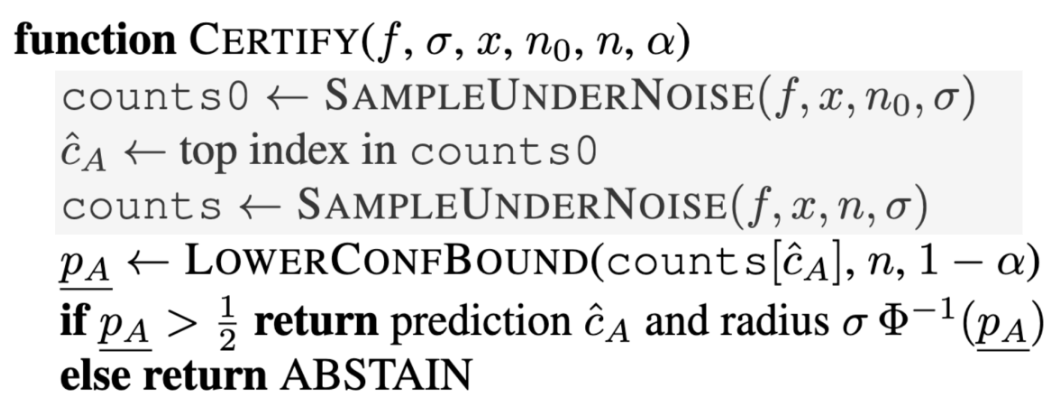
\includegraphics[width=\columnwidth]{img/rand_smooth.png}

At inference time, to compute $g(x)$, we need another sampling procedure:

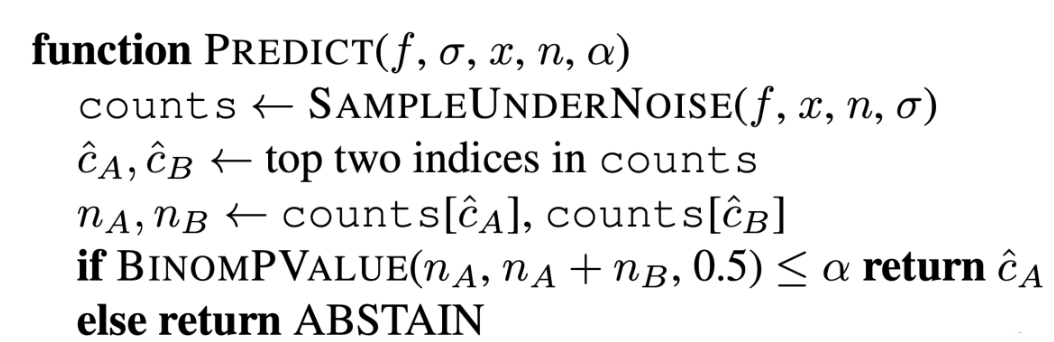
\includegraphics[width=\columnwidth]{img/rand-predict.png}

The probability of wrong prediction is $P(\hat{c_A}\ne c_A, \text{no abstain}) = P(\hat{c_A}\ne c_A)P(\text{no abstain} \mid \hat{c_A}\ne c_A) \le \alpha$.

Pros: (1) it can scale to large networks and (2) is model-agnostic.

Cons: (1) it requires sampling at inference time and (2) many samples could be needed to increase the certified radius.